\documentclass[../Main.tex]{subfiles}

\begin{document}

\section{Newmark Beta Methods}

In this  section, we will look at a family of numerical methods used to solve second order ordinary differential equations. We will look at the general formula, the algorithm to implement them, and an experimental verification of convergence order for different values of the parameters.

\subsection{Introduction to Newmark Beta Methods}\label{subsection:intro_newmark-beta}
The Newmark Beta methods were presented by Nathan M. Newmark in a paper \cite{Newmark1959} published in 1959. They were intended to be used for find solutions to problems in structural dynamics, \textit{``capable of application to strucutres of any degree of complication, with any relationship between force and displacement''}, with considerations for \textit{``any time of dynamic loading such as that due to shock or impact, vibration, earthquake motion, or blast from a nuclear weapon''}. However, they can also be used in less apocalyptical scenarios -  with a special case known as the `Velocity Verlet' algorithm being the standard for solving the equatoins of motion in molecular dynamics simulations.
Writing $\vec{x}_{i}$, $\vec{v}_{i}$, and $\vec{a}_{i}$ for the displacement, velocity, and acceleration at timestep \textit{i} respectively, the methods are of the form:
\begin{align}
	\begin{split}
		\vec{v}_{i+1} & = \vec{v}_{i} + h\left[\left(1-\gamma \right)\vec{a}_{i} + \gamma \vec{a}_{i+1}\right] \\
		\vec{x}_{i+1} & = \vec{x}_{i} + h\vec{v}_{i} + \frac{h^2}{2}\left[ \left(1-2\beta \right)\vec{a}_{i} + 2\beta \vec{a}_{i+1}\right] 
	\end{split} \label{eqn:newmark-beta}
\end{align} where $\gamma \in \left[0, 1 \right]$ and $2\beta \in \left[0, 1 \right]$.  

We have that the methods are second order accurate if and only if $\gamma = \frac{1}{2}$, and that they are conditionally stable if and only if $2\beta \geq \gamma \geq \frac{1}{2}$. The proof of these attributes is beyond the scope of this paper, and can be found in \cite{Newmark1952}. However, we will look at confirming the first statement through numerical simulations in Subsection~\ref{subsection:numerical_newmark-beta}. 

Some of the common choices of parameters $\beta$ and $\gamma$ are:
\begin{itemize}
	\item Average Acceleration Method $\left(\gamma = \frac{1}{2} \mbox{, } \beta = \frac{1}{4}\right)$:
\begin{align*}
	\vec{v}_{i+1} & = \vec{v}_{i} + h\left[\frac{1}{2}\vec{a}_{i} + \frac{1}{2}\vec{a}_{i+1}\right]\\
	\vec{x}_{i+1} & = \vec{x}_{i} + h\vec{v}_{i} + \frac{h^2}{2}\left[\frac{1}{2}\vec{a}_{i} +\frac{1}{2}\vec{a}_{i+1}\right]
\end{align*}
	\item Linear Acceleration Method $\left(\gamma = \frac{1}{2} \mbox{, } \beta = \frac{1}{6}\right)$:
\begin{align*}
	\vec{v}_{i+1} & = \vec{v}_{i} + h\left[\frac{1}{2}\vec{a}_{i} + \frac{1}{2}\vec{a}_{i+1}\right]\\
	\vec{x}_{i+1} & = \vec{x}_{i} + h\vec{v}_{i} + \frac{h^2}{2}\left[\frac{2}{3}\vec{a}_{i} +\frac{1}{3}\vec{a}_{i+1}\right]
\end{align*}
	\item Velocity Verlet Method $\left(\gamma = \frac{1}{2} \mbox{, } \beta = 0\right)$:
\begin{align}
	\begin{split}
	\vec{v}_{i+1} & = \vec{v}_{i} + h\left[\frac{1}{2}\vec{a}_{i} + \frac{1}{2}\vec{a}_{i+1}\right] \\
	\vec{x}_{i+1} & = \vec{x}_{i} + h\vec{v}_{i} + \frac{h^2}{2}\vec{a}_{i}
	\end{split} \label{eqn:velocity_verlet}
\end{align}
\end{itemize}
\subsection{Computational Application of Newmark Beta Methods} \label{subsection:numerical_newmark-beta}
Figure~\ref{fig:newmark-beta_algorithm_original} shows an excerpt from the original manuscript \cite{Newmark1959} where Newmark outlines an algorithm to calculate the next values. The method suggested belongs to a class of methods known as `predictor-corrector' methods - an initial `predicition' of the quantity at $t_{i+1}$ is calculated using some function, and then this value is `corrected' by using the prediction as the initial value for some other function to calculate the value of the quantity at the same point in time, $t_{i+1}$. The example below depicts the Heun method for an ODE of the form $y' = f\left(t\mbox{, }y\right), \quad y\left(t_{0}\right) = y_{0}$.
\begin{align*}
	\tilde{y}_{i+1} & = y_{i} + hf\left(t_{i}\mbox{, }y_{i}\right) & \mbox{prediciting using Forward Euler Method} \\
	y_{i+1} & = y_{i} + \frac{h}{2}\left(f\left(t_{i}, y_{i}\right) + f\left(t_{i+1}, \tilde{y}_{i+1}\right)\right). & \mbox{correcting using Trapezium Rule}
\end{align*}
However, this raises a question: how many times should the cycle of prediction and correction be run to get an accurate result? We can avoid this question by simplifying our assumptions. Since the goal of this paper is to apply the Newmark Beta methods to a molecular dynamics simulation, we can tune the method accordingly. In the absence of external forces, the molecular dynamics simulation is a conservative system. So the force (and by Newton's Second Law, the acceleration) is dependent only on the displacement of the particles. Thus, we can re-write Equation\ref{eqn:newmark-beta} as:
\begin{align*}
	\begin{split}
		\vec{v}_{i+1} & = \vec{v}_{i} + h\left[\left(1-\gamma\right)\vec{a}_{i} + \gamma\vec{a}_{i+1}\left(\vec{x}_{i+1}\right)\right] \\
		\vec{x}_{i+1} & = \vec{x}_{i} + h\vec{v}_{i} + \frac{h^2}{2}\left[\left(1-2\beta \right)\vec{a}_{i} + 2\beta\vec{a}_{i+1}\left(\vec{x}_{i+1}\right)\right] 
	\end{split}
\end{align*}
as we will already have computed the values of $\vec{x}_{i}, \vec{v}_{i},\mbox{ and }\vec{a}_{i}$.
\begin{figure}[h]
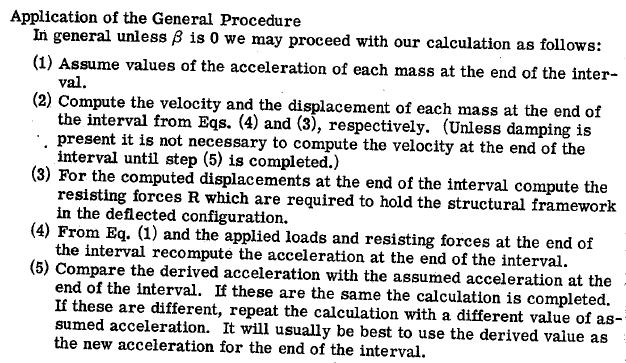
\includegraphics{newmark-beta_algorithm_original}
\centering
\caption{Excerpt on applying the Newmark Beta methods computationally}
\label{fig:newmark-beta_algorithm_original}
\end{figure}

Thus, we can see that the equation is implicit for $\vec{x}_{i+1}$. However, it is explicit for $\vec{v}_{i+1}$, as we can calculate $\vec{a}_{i+1}$ once we have the value of $\vec{x}_{i+1}$.  We use Newton-Raphson Iteration to solve for $\vec{x}_{i+1}$:
\begin{align}
	\vec{\tilde{F}}\left(\vec{x}_{i+1}\right) & = \vec{x}_{i+1} - \vec{x}_{i} -h\left(\vec{v}_{i} + \frac{h}{2}\left(\left(1-2\beta\right)\vec{a}_{i} + 2\beta\vec{a}_{i+1}\left(\vec{x}_{i+1}\right)\right)\right) \nonumber \\
	D_{\vec{x}_{i+1}}\vec{\tilde{F}}\left(\vec{x}_{i+1}\right) & = \textbf{I} -  \beta h^{2}\textbf{J}_{\vec{a}_{i+1}} \nonumber \\
	\vec{x}_{i+1} & = \vec{x}_{i} - D\vec{\tilde{F}}\left(\vec{x}_{i}\right)^{-1}\vec{\tilde{F}}\left(\vec{x}_{i}\right) \label{eqn:newton-raphson_final_step}
\end{align}
provided that the inverse exists. Thus, we use the following algorithm to find the next set of points: \\
\begin{algorithm}[H]
\SetAlgoLined
\SetKwInOut{Input}{input}\SetKwInOut{Output}{output}

\Input{$\vec{x}_{i},\vec{v}_{i}, \vec{a}_{i}, h, \gamma, \beta$}
\Output{$\vec{x}_{i+1}, \vec{v}_{i+1}, \vec{a}_{i+1}$}
\BlankLine

$\vec{v}_{i+1} \leftarrow \vec{v}_{i} + h\left(1-\gamma\right)\vec{a}_{i}$\\
Calculate $\vec{x}_{i+1}$ using the Newton-Raphson Method \\
$\vec{a}_{i+1} \leftarrow \frac{1}{m}\vec{F}\left(\vec{x}_{i+1}\right)$\\
$\vec{v}_{i+1} \leftarrow \vec{v}_{i+1} + \gamma h\vec{a}_{i+1}$ \tcp*{Splitting the update into two steps to reduce space usage}
\caption{Newmark-Beta Method Algorithm}
\label{algorithm:newmark-beta}
\end{algorithm}
\BlankLine
Now that we have the algorithm laid out, we can look at applying it to an example and test the convergence of Newmark Beta methods.

\subsection{Convergence Tests}

We consider the case of a pendulum, governed by the equation:
\begin{align}
\frac{d^2\theta}{dt^2} = -\frac{g}{l}\sin(\theta)
\end{align}

We test for convergence in the following way: we fix $T = 5$, $\beta$ and $\gamma$, and consider $N = 16, 32, 64, 128, 256, 512, \mbox{and } 1024 \left(\mbox{hereby varying } h := \frac{T}{N}\right)$. Then, for each value of $h$, we calculate the position and velocity of the pendulum at $T = 5$, and compare these values to the reference solution calculated using MATLAB's \texttt{ode45} function. We define the overall error in the estimation at time $t_{i}$ as a function of the error in displacement and velocity at $t_{i}$:
\begin{align*}
err_{i} = \sqrt{\left(err_{x_{i}}\right)^2 + \left(err_{v_{i}}\right)^2}
\end{align*}
Looking at the Taylor series expansion of the analytical solution, we get that $err_{i} \approx \mathcal{O}\left(h^a\right)$ for some $a \in \mathbb{Z}^{+}$. Hence, we get that $a$ - the order of convergence - will the gradient of the straght line when $\log\left(err_{i}\right) \mbox{is plotted against} \log\left(h\right)$. We can see that Figure~\ref{fig:newmark-beta_convergence} corroborates the statement in Subsection~\ref{subsection:intro_newmark-beta} - the order of a Newmark Beta method is 1 unless $\gamma = 0.50$, when it is $2$.

\begin{figure}[H]
\centering
 	\begin{tabular}{@{}cc@{}}
		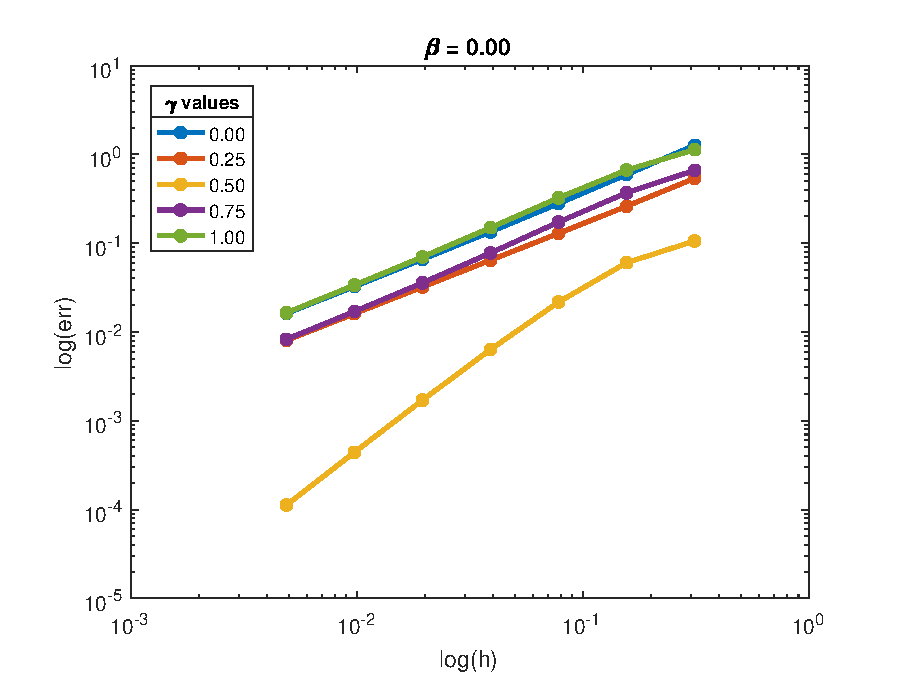
\includegraphics[width=0.5\textwidth]{convergence_beta_0,00.eps} &
    		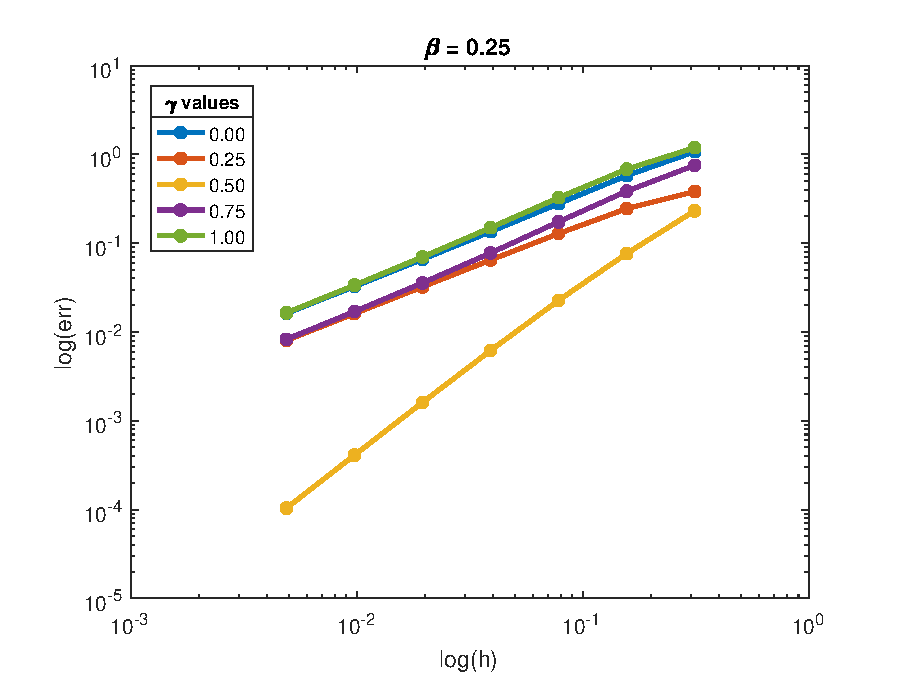
\includegraphics[width=0.5\textwidth]{convergence_beta_0,25.eps} \\
    		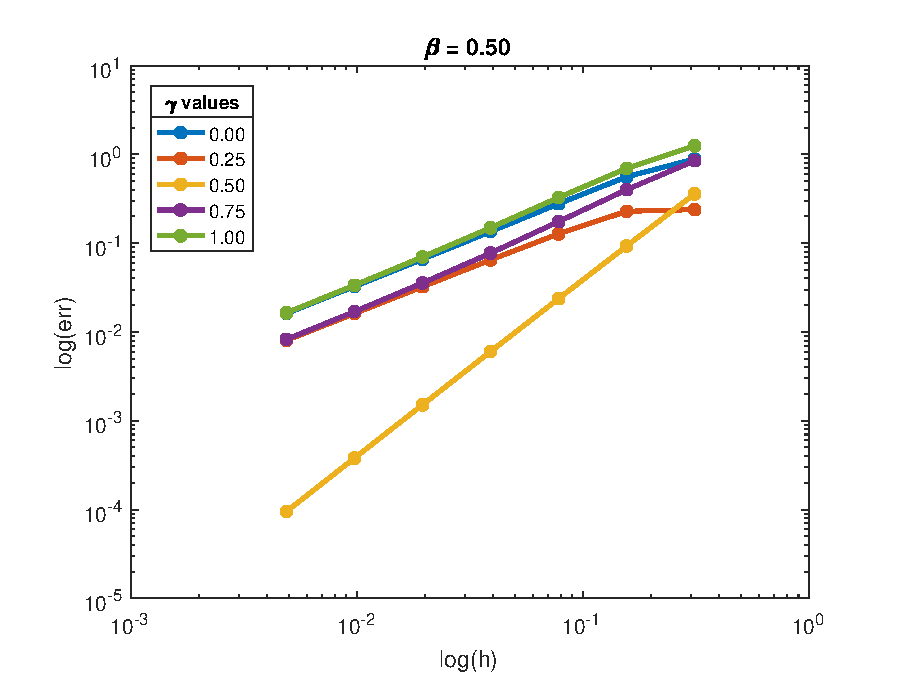
\includegraphics[width=0.5\textwidth]{convergence_beta_0,50.eps} &
   		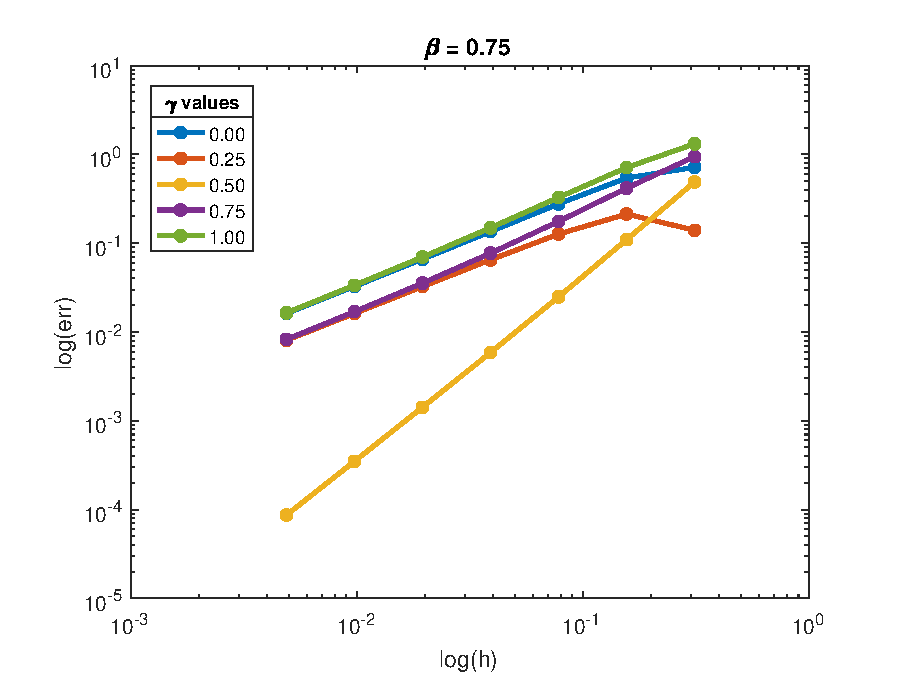
\includegraphics[width=0.5\textwidth]{convergence_beta_0,75.eps} \\
    		\multicolumn{2}{c}{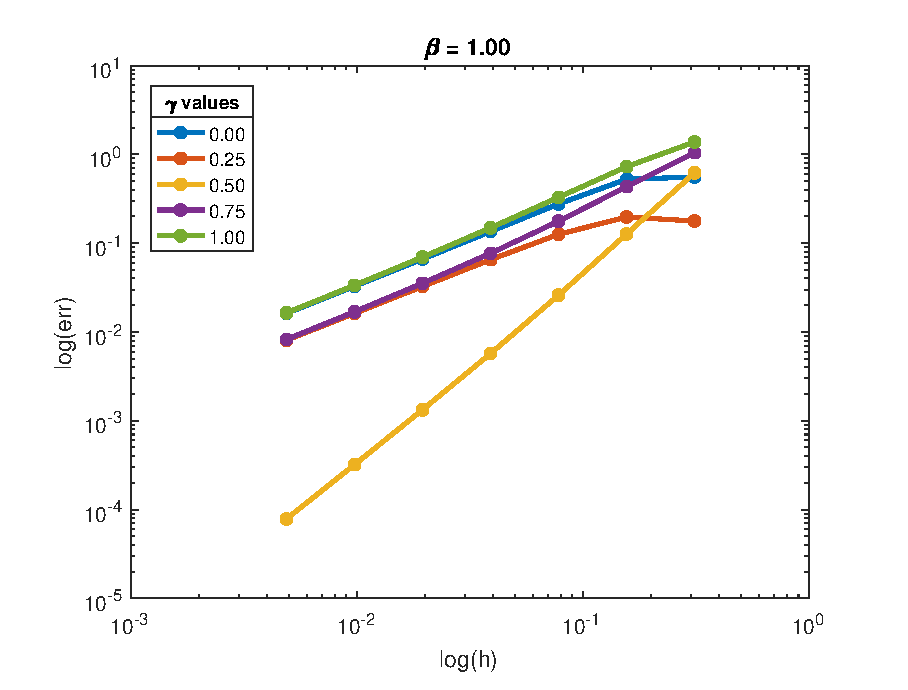
\includegraphics[width=.5\textwidth]{convergence_beta_1,00.eps}}
  	\end{tabular}
  	\caption{Order of convergence of Newmark Beta methods for varying parameter values}
	\label{fig:newmark-beta_convergence}
\end{figure}
\end{document} 